\documentclass{article}
\usepackage{amsmath}
\usepackage{graphicx}
\usepackage{biblatex} %Imports biblatex package
\addbibresource{sample.bib} %Import the bibliography file

\title{Report for Deep Generative view on Continual Learning
Project\\[1cm]Riccardo Ceccaroni}

\begin{document}
\maketitle


\section{Introduction}
This project aims to develop a generative replay method for continual learning using Generative Adversarial Networks (GANs) as the generative model \cite{Goodfellow2014GAN}. The goal is to evaluate this method in a class-incremental learning scenario, where the MNIST dataset \cite{LeCun1998MNIST} is divided into five tasks, each containing two classes. This approach addresses the challenge of catastrophic forgetting by generating replay samples for previously learned tasks, allowing the model to retain knowledge over time \cite{Shin2017Continual, Wu2018MemoryReplay}.

In a class-incremental scenario, the model sequentially learns new classes without revisiting old data. The generative replay method leverages GANs to produce samples from past tasks, which are then used during training on new tasks to maintain performance on earlier tasks. The effectiveness of this method will be assessed using three metrics: average accuracy, forward transfer (FWT), and backward transfer (BWT) \cite{LopezPaz2017GEM, Chaudhry2018RWalk, DiazRodriguez2018DONUT}. 

\section{Methods}

\subsection{Model Architecture}
The neural network model used is a Multi-Layer Perceptron (MLP) with three hidden layers. Each hidden layer consists of 50 neurons with ReLU activation functions. In addition, we employ a GAN to generate replay samples, helping the model retain knowledge from previous tasks.

The \texttt{Agent} class handles the training and validation of the model, managing the learning process across multiple tasks.
The \texttt{Agent} is initialized with the model, optimizer, loss criterion, and datasets. An optional parameter allows the use of a vanilla model or a model augmented with a GAN for memory replay.
The training process involves iterating over each task and training the model using the respective task dataset. For the GAN-augmented model, replay samples are generated and mixed with current task data to prevent forgetting previous tasks.
Validation is performed periodically to evaluate the model's performance on each task. Accuracy is recorded at the end of each epoch and task.

\subsection{Metrics}
The model's performance is evaluated using several metrics, including average accuracy, backward transfer (BWT), and forward transfer (FWT).
\begin{itemize}
    \item Accuracy: is a performance metric used to evaluate the effectiveness of a classification model. It is defined as the ratio of the number of correct predictions made by the model to the total number of predictions.

    \item BWT: measures the influence of learning new tasks on the performance of previously learned tasks. It is computed by comparing the end-of-training accuracy of each task with its accuracy immediately after training on the task.
    
    \item FWT: measures the influence of learning previous tasks on the performance of new tasks. It is computed by comparing the initial accuracy of each task with the model's accuracy on the same task when it was first encountered.
\end{itemize}

\subsection{Dataset}
The MNIST dataset is used, consisting of 60,000 training images and 10,000 test images of handwritten digits (0-9). The dataset is divided into tasks, each containing data from a subset of the digit classes.
%
The MNIST dataset is loaded using the \texttt{mnist} module, which initializes and loads the training and test data into \texttt{x\_train}, \texttt{t\_train}, \texttt{x\_test}, and \texttt{t\_test} variables.
%
Tasks are created by splitting the dataset into subsets, each corresponding to a specific set of classes. The tasks are generated using the \texttt{get\_dataset} function, which shuffles the classes and assigns them to different tasks. This function returns the training and validation datasets for each task.
%
The function \texttt{get\_iter\_dataset} extracts data points belonging to a specific class from the dataset, facilitating the creation of subsets for each task.




\section{Results}
This section compares the results obtained using the vanilla versus the GAN-based approach. 

In the vanilla method, all images from the previous task are stored and used for training the next task. Conversely, the GAN method involves training a single GAN network on the previous tasks to generate samples for predicting the total learning loss on those tasks.

The hyperparameters for training the classifier are the same for both methods: a learning rate of $1e^{-5}$, a batch size of $128$, and $50$ epochs on a $3$-layer MLP with a hidden layer size of $256$. A small learning rate is set to prevent the loss of previously acquired information. For the GAN, $1000$ samples are generated from the previous tasks.

The results (Figure \ref{fig:1} vs Figure \ref{fig:3}) indicate that the GAN-based method yields lower accuracy. This lower performance may be due to several factors, primarily that the generated samples from previous tasks are fewer than the actual dataset in the vanilla method. Additionally, the generated dataset might be imbalanced, leading to a decrease in accuracy for certain classes, such as class 1 (Figure \ref{fig:2} vs Figure \ref{fig:4}), with each iteration. Suggestions for improving the architecture to achieve better accuracy are provided in Section \ref{sec:improving}.

\subsection{Vanilla}
The average accuracy at the end of the sequence is $0.973$, with a Backward Transfer (BWT) of $-0.002$ and a Forward Transfer (FWT) of $-0.126$.

\begin{figure}[h!]
\centering
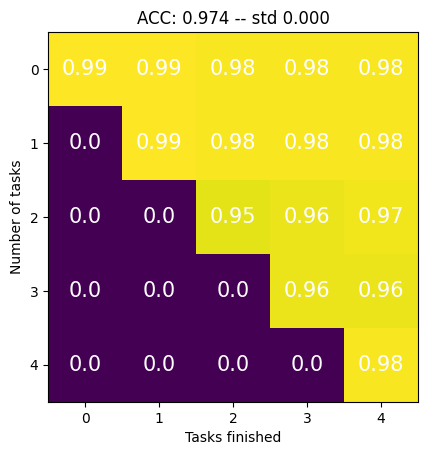
\includegraphics[width=8cm]{imgs/vanilla1.png}
\caption{Accuracy matrices showing the performance on each task after each epoch}
\label{fig:1}
\end{figure}
\begin{figure}[h!]
\centering
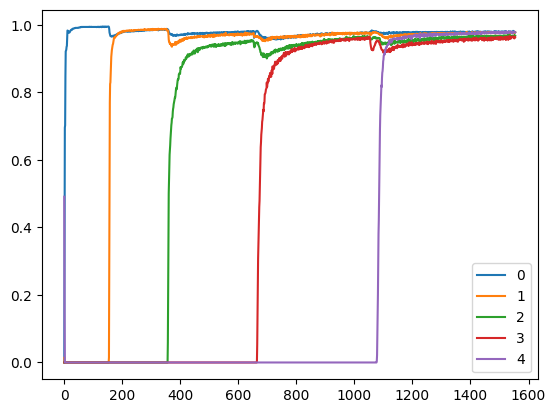
\includegraphics[width=8cm]{imgs/vanilla2.png}
\caption{Accuracy-over-time plots illustrating the model's performance across tasks over time}
\label{fig:2}
\end{figure}

\subsection{GAN}
The average accuracy at the end of the sequence is $0.724$, with a Backward Transfer (BWT) of $-0.319$ and a Forward Transfer (FWT) of $-0.127$.

\begin{figure}[h!]
\centering
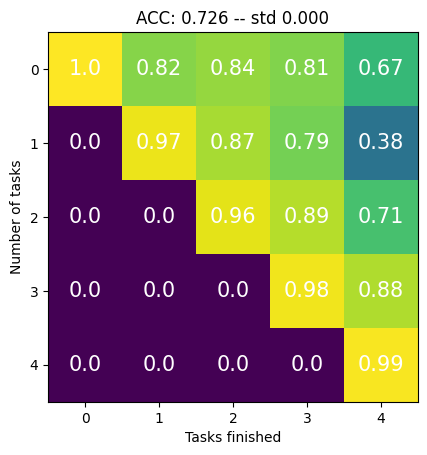
\includegraphics[width=8cm]{imgs/gan1.png}
\caption{Accuracy matrices showing the performance on each task after each epoch}
\label{fig:3}
\end{figure}
\begin{figure}[h!]
\centering
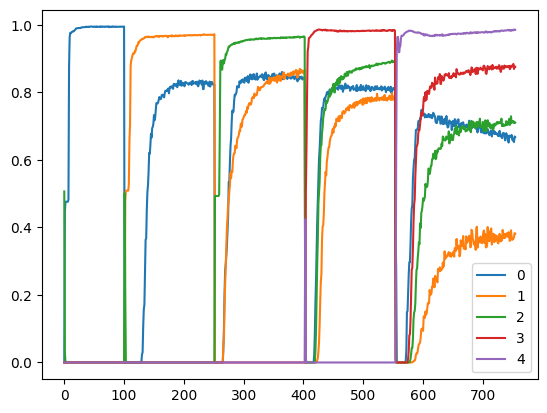
\includegraphics[width=8cm]{imgs/gan2.png}
\caption{Accuracy-over-time plots illustrating the model's performance across tasks over time}
\label{fig:4}
\end{figure}




\section{Discussion}

\subsection{Memory Requirements}
The memory requirements for both the generative replay and vanilla replay approaches involve storing data for past tasks to mitigate catastrophic forgetting. In vanilla replay, raw samples from previous tasks are stored. If each task contains \(m\) samples, and each sample is represented by a vector of size \(d\), the memory required for \(n\) tasks is calculated as:
\[
\text{Memory}_{\text{vanilla}} = n \times m \times d
\]

In generative replay, a GAN is used to generate samples from previous tasks. The memory required includes the model parameters of the GAN and the neural network used for classification. Let \(p_{\text{GAN}}\) be the number of parameters in the GAN and \(p_{\text{model}}\) be the number of parameters in the classification model. The memory required for \(n\) tasks is:
\[
\text{Memory}_{\text{generative}} = p_{\text{GAN}} + p_{\text{model}}
\]

In practice, the memory required for storing the model parameters (GAN and classification model) is often significantly less than storing raw samples for each task, especially as the number of tasks (\(n\)) increases.

\subsection{Computational Requirements}
In terms of memory, generative replay can be more efficient than vanilla replay, particularly for large \(n\). Computationally, both approaches scale with the number of tasks, but generative replay introduces extra computational overhead due to sample generation.

For vanilla replay, the computational cost is proportional to the number of samples replayed during training. Each replay involves a forward and backward pass through the classification model:
\[
\text{Computation}_{\text{vanilla}} \propto n \times m
\]

Generative replay involves generating samples using the GAN, followed by a forward and backward pass through the classification model. The computational cost for generating samples and training is:
\[
\text{Computation}_{\text{generative}} \propto \text{GAN}_{\text{generation}} + n \times m
\]
where \(\text{GAN}_{\text{generation}}\) denotes the cost of generating samples using the GAN. Although generating samples introduces additional computation, the generative approach can be more efficient if the GAN is trained effectively and the generation cost is lower compared to storing and replaying a large number of raw samples.


\subsection{Scalability with Number of Tasks}
Vanilla replay exhibits linear scalability in both memory and computational requirements with the number of tasks.
Generative replay, on the other hand, is less sensitive to the number of tasks in terms of memory requirements, primarily depending on the model parameters.
However, the computational requirement scales linearly with the number of tasks, with an added constant cost for generating samples.

\subsection{Downsides of the Approach}
Generative replay has several downsides. The quality of generated samples heavily depends on the effectiveness of the GAN, and poor sample quality can degrade the model's performance. Additionally, generating samples introduces extra computational cost, which can be significant depending on the complexity of the GAN. Training GANs can be challenging and unstable, requiring careful tuning and potentially more computational resources.

Vanilla replay also has its limitations. Storing raw samples for each task can lead to high memory usage, especially as the number of tasks increases. Furthermore, the linear increase in memory and computational requirements can make vanilla replay infeasible for a large number of tasks.

\subsection{Improving Efficiency}
\label{sec:improving}
To improve the accuracy of the presented architecture, several enhancements can be made. Increasing the number of samples generated by the GAN for previous tasks is one approach. Additionally, upgrading the classifier to a convolutional network could enhance performance. To address dataset imbalance, a separate GAN can be trained for each previous task, allowing multiple GAN generators to create samples from those tasks.

Furthermore, memory efficiency can be improved by generating GAN samples in batches rather than all at once. This method enables processing each batch with the classifier sequentially, thereby allowing a large number of samples to be generated without significantly impacting memory usage.

To enhance memory efficiency, techniques like sample compression can be employed. This involves using methods such as quantization or autoencoders to compress the raw samples, thereby reducing the memory footprint. Another approach is selective storage, where only a subset of representative samples from each task is stored, minimizing memory usage while maintaining performance.

For improving computational efficiency, efficient GAN training methods can be utilized. Techniques such as progressive GANs or lightweight GAN architectures can help reduce the computational cost of generating samples. Additionally, hybrid approaches can be considered, combining generative replay with other efficient replay methods like rehearsal with synthetic samples to balance memory and computational efficiency. Incremental learning techniques can also be implemented, allowing the model to adapt to new tasks without extensive replay of old tasks, thus reducing overall computational requirements.


\section{Conclusion}
The generative replay method utilizing GANs for continual learning was implemented and evaluated on the MNIST dataset in a class-incremental learning scenario. The dataset was split into five tasks, each containing two classes. The evaluation focused on three key metrics: average accuracy, FWT, and BWT.

The results indicate that the generative replay method can mitigate catastrophic forgetting and maintain performance across multiple tasks. The average accuracy demonstrates the model's overall competence, while the FWT and BWT metrics provide insights into the transfer of knowledge between tasks. 

The approach has some downsides, including computational overhead from generating replay samples and potential instability in GAN training. Future improvements could focus on enhancing memory and computational efficiency, such as using sample compression, selective storage, efficient GAN architectures, hybrid approaches, and incremental learning techniques.

\printbibliography %Prints bibliography


\end{document}
